%!TEX root = ../template.tex
%%%%%%%%%%%%%%%%%%%%%%%%%%%%%%%%%%%%%%%%%%%%%%%%%%%%%%%%%%%%%%%%%%%%
%% chapter2.tex
%% NOVA thesis document file
%%
%% Chapter with the template manual
%%%%%%%%%%%%%%%%%%%%%%%%%%%%%%%%%%%%%%%%%%%%%%%%%%%%%%%%%%%%%%%%%%%%

\typeout{NT FILE chapter2.tex}%

\chapter{Background}\label{cha:Background}

In this chapter we will discuss relevant work considering the goals of the work
to be conducted in this thesis. In particular, we will focus on the following topics:

In Section~\ref{sec:membership_protocols} we discuss the differences between
the different kinds of membership systems as well as some implementations.

In Section~\ref{sec:consensus} we will discuss some consensus protocols.

In Section~\ref{sec:blockchain} we will discuss some different types of
blockchain protocols.

\section{Membership Protocols}\label{sec:membership_protocols}

This section introduces membership protocols that have been considered to
be implemented as part of the work that will be developed. We selected these
memberships to study due to their wide differences in properties and their
popularity in usage.

\subsection{Membership}\label{sub:membership}

A protocol where each node knows every other node in the network might work well
for small networks, but it is not a scalable solution since each node would need
to have \textit{n - 1} communications channels open at all time, being n the
amount of nodes in the system, and each node needs to be following any and all
changes to the system. This is not feasible since the number of links between
nodes would rise quadratically and networks can easily reach thousands of
participants. In order to overcome the challenges that arise from large networks,
we usually use partial view membership protocols. In these protocols each node only knows
and maintains information about a small selection of nodes in the systems,
making it a more scalable strategy than a total view protocol, since
the number of connections tend to grow at a logarithmic rate instead.

When maintaining a partial view, protocols usually follow one of two strategies
when managing their memberships:

\begin{itemize}
  \item \textbf{Reactive:} Using this strategy, the partial view undergoes alteration solely
when there are changes in membership, typically occurring when a node joins or leaves the membership.
  \item \textbf{Cyclic:} With this approach, the partial view changes periodically.
Every \textit{t} seconds nodes exchange information that may lead to modifications to the
partial view.
\end{itemize}

This membership protocols are usually represented by a graph where the vertices represent
the participants of the network and the edges represent the communication links.
Depending on how the graph ends up we can classify the membership as structured,
unstructured or partially structured. In the next sections we will go over these
types of memberships and some implementations.

\subsection{Structured Overlays}\label{sub:structured_overlays}

Structured overlay memberships follow a pre-defined structure by having the nodes
routed to a specific logical position in the network. This known structure allows
improvement on search primitives, enabling efficient discovery of data and process.
The node's position is usually based on a unique identifier for each node of the
network and different protocols organize the nodes by their identifier by 

However, having a predefined topology come at the cost of a more costly re-structuration
of the network every time a there is a change to the membership. This process
is usually slow and costly since a change of one node may affect
the network at a global level. This drawback becomes more relevant in high churn rate
scenarios.

\subsubsection{Chord}\label{subsec:chord}

Consistent Hashing and Random Trees, or Chord~\cite{chord} is a Distributed Hash
Table based algorithm where each node is assigned a unique identifier based on
the output of a cryptographic hash function like SHA-1 or MD-5. Usually this hash is based on the IP address of
the node since this is unique for every node of the network, and making it so
that once a node joins the network their identifier is set in stone. These
identifiers determine key assignment in the distributed hash table: each node is responsible
for all keys in the range from its predecessor's identifier (exclusive) to its own identifier (inclusive).
More formally, a node with identifier \textit{n} is responsible for keys in the range \textit{]predecessor(n), n]}.
This ensures that every possible key in the identifier space is assigned to exactly one node,
with keys hashed using the same hash function used for node identifiers.

The graph generated based on the membership overlay will be a cyclic graph with
a ring shape, with the nodes ordered by their generated identifier and each node maintains a direct link
to their predecessor and successor. Each node
also maintains a routing table with around O(\textit{log n}) distinct entries
called a finger table. Using this routing table we can improve the lookups from O(\textit{n}) to O(\textit{log n})
since we can search in our finger table for the node with the closest preceding identifier instead of
navigating the ring node by node.

The tables maintained by these nodes are automatically updated when a new node joins
or leaves the system  making it always possible to find a node responsible to a given
key. However, simultaneous failures may break the overlay since the correctness
of the membership depends on each node knowing their correct neighbors. In order
to increase fault tolerance, a periodical stabilization protocol is run in background,
making sure the neighbors are still active and restructuring the overlay
accordingly as well as updating the entries on the finger table.

\subsubsection{Pastry}\label{subsec:pastry}

Pastry~\cite{pastry}, similarly to Chord is a structured overlay protocol that
defines a distributed hash table. A Pastry system is a self-organizing overlay
network of nodes where every node has a 128-bit identifier. This identifier
is assigned randomly when a node joins the system and is used to indicate a
node's position in a circular space that ranges from 0 to $2^{128}-1$. It is assumed
that the hash function that gives the node's identifier generated a uniform
distribution of identifiers around the 128-bit space.

Each Pastry node maintains a \textit{routing table}, a \textit{neighborhood set}
and a \textit{leafing set}. The routing table is organized in levels, where each level
\textit{l} contains entries for nodes that share an \textit{l}-digit prefix with the local
node's identifier, typically using base-$2^b$ encoding (commonly b=4), the routing
table has up to $2^b$ entries per level, allowing efficient prefix-based routing.

The neighborhood set contains the \textit{M} nodes that are closest to the local node in
terms of network proximity (measured by latency or network distance), not identifier space proximity.

The leaf set contains the \textit{L}/2 numerically closest nodes with smaller identifiers and \textit{L}/2
numerically closest nodes with larger identifiers in the circular identifier space.

When a new node joins, it contacts an existing nearby node and obtains initial routing state by querying
nodes along the path to its final position and updates routing tables, leaf sets,
and neighborhood sets of affected nodes. 

Pastry runs periodic maintenance protocols to ensure routing correctness. Nodes periodically exchange
keep-alive messages with their leaf set and neighborhood set members, update routing table entries by probing
nodes with longer common prefixes, and repair any detected inconsistencies in their routing state when there are changes
in the membership.

Pastry uses a three-step routing algorithm: (1) if the destination is within the leaf set range,
route directly to the destination or the numerically closest node; (2) if not, forward to a node from
the routing table that shares a longer common prefix with the destination; (3) if no such node exists,
forward to a node from the leaf set or neighborhood set that is numerically closer to the destination.
With this algorithm Pastry achieves O(\textit{log N}) expected routing hops for message delivery and maintains
O(\textit{log N}) routing state per node, making it highly scalable for large networks.


\subsection{Unstructured Overlays}\label{sub:unstructured_overlays}

Unstructured overlays place few constrains as on how the nodes chose their
neighbors. This results in a random graph that is hard to predict and describe.

By not having a structured overlay these memberships end up being more fault-tolerant
in high churn rate scenarios due to the cost of the network restructuring
itself is fairly low.

\subsubsection{SWIM}\label{subsec:swim}

SWIM~\cite{swim} stands for \textbf{S}calable \textbf{W}eakly-consistent \textbf{I}nfection-style
Process Group \textbf{M}embership Protocol. This protocol is composed of two distinct
components, a failure detector and a dissemination component.

Unlike traditional gossip based overlays that rely on a heartbeat strategy,
the failure detector in SWIM is independent of the rest of the protocol.
The failure detector is fully decentralized and is executed in a randomized
probe-based fashion, the authors later suggest an optimization via a round-robin
fashion instead.

SWIM uses a three-state model for nodes: alive, suspect, and failed. When a direct probe fails,
the target node enters the suspect state rather than being immediately marked as failed.
During the suspicion period, other nodes can refute the suspicion by providing evidence
that the suspected node is actually alive. This mechanism significantly reduces false positives
while maintaining rapid failure detection.

SWIM uses incarnation numbers to handle false suspicions: each node maintains an incarnation
number that it can increment to refute suspicions about itself. The protocol uses specific
message types including \textit{PING} (direct probe), \textit{PING-REQ} (indirect probe request), \textit{ACK} (acknowledgment),
and membership update messages that carry node states and incarnation numbers.

The other component of this protocol is the gossip dissemination system which
maintains a partial view of the network. This component updates whenever a member
joins or leaves the system by an infection style dissemination protocol. In order to
make this more efficient, the updates piggyback the messages that are sent during the
failure detection procedure.

SWIM achieves excellent scalability properties: failure detection time is O(\textit{1}) with respect to group size,
and each node generates a constant message load per time period regardless of the total number of nodes.
The protocol provides eventual consistency of membership views across all nodes, new nodes join
by contacting any existing member and receiving their current membership list. The weak consistency model
ensures that all correct nodes eventually converge to the same membership view, though temporary
inconsistencies may exist during high churn periods.

\subsubsection{HyParView}\label{subsec:hyparview}

HyParView~\cite{hyparview} is a gossip based membership protocol that offers high
resilience and high delivery reliability of messages while being highly scalable.
It relies on a hybrid approach by maintaining two distinct views: an \textit{active view}
used for reliable message dissemination, and a \textit{passive view},
usually 3 to 5 times larger than the active view,
that serves as a backup for network restructuring when the active view changes.

HyParView uses different approaches when it comes to maintaining each of the views,
for active view a reactive strategy is used, nodes react to events that require 
the network to be restructured such as new nodes joining the membership or
existing ones leaving, either by failing or by choice.

The nodes in the active view are the ones with which each node maintains a
communication link. In case the active view needs to be changed the nodes in
the passive view may be promoted to active nodes the same way nodes in the
active view may be demoted to the passive view. All the nodes in the active
view of a given node have that node in their active view, making the connection
graph that represents the overlay be a bidirectional graph.

For the passive view, HyParView uses a cyclic strategy with periodic shuffle operations
every \textit{t} seconds (typically 10-30). During a shuffle, a node exchanges
a subset of its passive view with a randomly selected active neighbor.
The neighbor responds with its own partial passive view. Both nodes
integrate received entries while maintaining view size limits through age-based eviction.
This mechanism ensures O(\textit{log N}) mixing time for achieving uniform random sampling
across the network and maintains connectivity with high probability.

The protocol uses TCP connection failures as an implicit failure detector: when a TCP
connection to an active neighbor fails, the node immediately replaces it by promoting
a node from the passive view to maintain the target active view size, providing
excellent fault tolerance properties and avoiding partitions even under high churn rates.

Tests done in \cite{hyparview} show that the algorithm is able to recover from as much as 80\%
node failure, as long as the overlay stays connected. By being able quickly react to failures
in the system, the protocol was shown to be able to maintain 100\% reliability 
for message dissemination.


\subsection{Partially Structured Overlays}\label{sub:partially_structured_overlays}

Partially structured overlays aim to get the best of both strategies. We can 
leverage the easy to maintain and fault-tolerant unstructured overlays and
by applying some optimization procedure to the network we can achieve a more
efficient search and application level routing.

\subsubsection{T-MAN}\label{subsec:t-man}

T-MAN~\cite{tman} was created with the motivation to give
the ability of taking some random overlay, and \textit{evolve} it into another one.

The logic behind the algorithm is giving each node a ranking value that every node can
use to apply a function to determine how desirable a node is as a neighbor.
Each node maintains a partial view that contains the addresses of nodes that are not its
immediate neighbors, much like the HyParView overlay described in \ref{subsec:hyparview}.
Periodically each node exchanges its partial view with the first node in its active view,
according to the ranking
values which depends on the target overlay. The receiver will execute the same procedure
as the sender, so they can later merge their local views and apply the ranking function.
Using their peers' views to improve their own the overlay will gradually become closer
the desired overlay.

Experimentally this algorithm is shown to be scalable and fast, with the convergence
times growing approximately at a logarithmic rate in function of the number of nodes in
the network. The problem that surges with this, is that the network only becomes as 
fault-tolerant as the desired overlay, since T-MAN doesn't aim to maintain a balanced degree
between the nodes, this might create uneven load balance or even node isolation during
or after the procedure

\subsubsection{X-BOT}\label{subsec:x-bot}

X-BOT~\cite{xbot} stands for \textbf{B}ias the \textbf{O}verlay \textbf{T}opology
according to some targeting criteria \textbf{X}. This protocol is completely decentralized,
and the nodes do not require any prior knowledge of where they will end up in the final topology. 
This protocol strives to preserve the degree of the nodes that participate in the 4-node coordinated
optimization technique, described in greater detail below, this is essential to preserve
the connectivity of the overlay. X-BOT is built in a way that every modification that is
done by the protocol increases its efficiency and due to the dynamic nature of the model,
its ensured that the overlay does not stabilize in a local minimum. These optimizations
are done in a way that key features of the overlay, such as low clustering coefficient and
low overlay diameter, are preserved. The protocol is highly flexible because it relies on a
companion oracle to estimate the link cost and therefore bias the network according to
different cost metrics.

The companion oracle is accessible by all nodes, and its sole purpose is to give the
link cost from the node that invokes it to a given node.

The 4-node coordinated technique that has been referred above works as follows, a
node \textit{i}, the initiator, starts the optimization round selecting a node from
its passive view. Node \textit{O} is a node from \textit{i}'s active view that
will be replaced. Node \textit{c}, the candidate, is a node from \textit{i}'s passive
view that is going to be upgraded to its active view. And finally node \textit{d}
is the node to be removed from the candidate's view so that \textit{i} can be accepted.
These nodes are always selected based upon the link cost values provided by the oracle,
ensuring that every time the optimization procedure is called the network increases its
efficiency.

\section{Consensus Protocols}\label{sec:consensus}

Consensus protocols are essential for the development of dependable distributed systems,
including replicated databases, distributed file systems and blockchain networks. They facilitate
the fundamental challenge of enabling distributed participants to reach agreement on a specific value.
These algorithms must guarantee that agreement is achieved in the presence of asynchronous communication
delays, network partitions, and defective nodes.

Any consensus protocol must satisfy the following properties~\cite{distributed_systems_concepts}:
\begin{itemize}
  \item \textbf{Termination:} Eventually, every correct process decides some value.
  \item \textbf{Agreement:} If all correct processes propose the same value \textit{v}, 
then any correct process that decides a value must decide \textit{v}.
  \item \textbf{Integrity:} No correct process decides more than once.
\end{itemize}

Consensus protocols differ on their assumptions about the system model's synchrony,
failure types and the number of faults
tolerated. FLP shows that deterministic consensus is 
impossible in asynchronous systems where there is at least one crash failure, making practical protocols
rely on additional assumptions like partial synchrony or randomization.

We will now examine specific protocols that solve consensus under different system models.

\subsection{Chandra-Toueg}\label{sub:chandra-toueg}

The Chandra-Toueg consensus protocol~\cite{chandra} solves consensus in partially synchronous
systems using an eventually strong failure detector.
This failure detector abstracts the timing assumptions needed for consensus, providing
an oracle that can make mistakes about process failures but eventually becomes reliable.
An eventually strong failure detector is defined by the following two properties:
\begin{itemize}
  \item \textbf{Strong Completeness:} Eventually, every process that crashes is permanently
  suspected by every correct process.
  \item \textbf{Eventual Strong Accuracy:} There is a time after which no correct process
  is suspected by any correct process (i.e., eventually the failure detector stops making
  false accusations about correct processes).
\end{itemize}

The algorithm operates in the crash-fault fail model, it assumes that fewer than half of the
processes can fail \textit{(f < n/2)} and guarantees termination in O(\textit{f+1})
rounds, where \textit{f} is the number of process failures. The protocol proceeds
in asynchronous rounds with a rotating coordinator selected in round-robin fashion. Each round consists of four phases:

\begin{enumerate}
  \item \textbf{Phase 1:} All processes send their current value and timestamp to the coordinator.
  \item \textbf{Phase 2:} The coordinator awaits to receive messages from a majority of processes.
  If successful, selects the value with the highest timestamp and broadcasts its chosen
  value to all processes. If the coordinator is suspected of failure, proceeds to the next round.
  \item \textbf{Phase 3:} Each process waits to receive the coordinator's proposal or for
  the failure detector to suspect the coordinator as failed:
  \begin{itemize}
    \item If the proposal is received then the process adopts it as its new value and sends
    an \textit{ACK} to the coordinator.
    \item If the coordinator is suspected of failure then the process sends a \textit{NACK} and proceeds
    to the next round with a new coordinator.
  \end{itemize}
  \item \textbf{Phase 4:} If the coordinator receives \textit{ACKs} from a majority of processes,
  it broadcasts a \textit{DECIDE} message with the chosen value. Upon receiving a \textit{DECIDE}
  message, processes decide on the value and terminate. The \textit{DECIDE} message is also
  relayed to ensure all correct processes eventually decide.
\end{enumerate}

\subsection{Paxos}\label{sub:paxos}

Paxos~\cite{paxos} is a family of protocols for solving consensus, for this example we will take
a look at what is commonly referred as basic Paxos, that decides on a single value, 
and after take a look at MultiPaxos which gives a constant stream of agreed values. 
For this algorithm we make the following assumptions regarding processors:
\begin{itemize}
  \item Operate at arbitrary seed.
  \item May experience failures.
  \item Have stable storage and may re-join the protocol after failures.
  \item Byzantine failures do not occur.
  \item The maximum number of failing processors is less than half of the total processors.
\end{itemize}
And the following assumptions regarding the network:
\begin{itemize}
  \item Processors can send messages to any other processor.
  \item Messages are asynchronous and take an arbitrary time to deliver.
  \item Messages may be lost, re-ordered or duplicate.
  \item Messages when delivered are delivered without corruption.
\end{itemize}

Each participant can act as a Proposer, an Acceptor and a Learner. Each execution 
of basic Paxos decides on a single value and operates in two phases, each with two
secondary phases.

\begin{itemize}
  \item \textbf{Phase 1}
  \begin{enumerate}
    \item \textbf{Prepare:} A Proposer creates a message which we call Prepare identified
with a number \textit{n}, this works as an identifier and has to be greater than
any previous number used in previous Prepare messages. The Prepare message does
not contain the proposed value. This message is sent to a quorum of acceptors, and
a proposer shouldn't initiate Paxos if it cannot communicate with a quorum of acceptors.
    \item \textbf{Promise:} Acceptors wait for a Prepare message from any of the proposers,
if they receive a message, depending on the value of \textit{n} two flows can happen:
    \begin{enumerate}
      \item If \textit{n} is higher than every previous proposal received from any Proposer
the Acceptor returns a Promise message and ignores all future proposals with a value
less than \textit{n}, if a proposal was accepted at some point in the past, the message
includes the previous \textit{n} value and the corresponding accepted value.
      \item Otherwise, the Acceptor can ignore the Prepare message or sending a not
acknowledge to tell the Proposer to stop its attempt to create the Proposal.
    \end{enumerate}
  \end{enumerate}

  \item \textbf{Phase 2}
  \begin{enumerate}
    \item \textbf{Accept:} If the Proposer receives Promises from a Quorum of Acceptors,
it sets a value for its proposal. If any Acceptors that accepted a previous proposal
they would have sent the previous accepted value, the Proposer will agree on the return
value sent by the Acceptors with the highest \textit{n}. In none of the acceptors had
previously accepted a value then the Proposer chooses the value it initially wanted to propose.
The proposer sends an Accept message with the chosen value and the \textit{n} value.
  \item \textbf{Accept:} If an Acceptor receives and Accept message from a Proposer,
it must accept if it hasn't proposed previously Proposals with an identifier grater than
\textit{n}. If the value is accepted, an Accepted message is sent to every proposer and Learner.
Learners will only learn the decided value after receiving Accepted messages from a majority
of Acceptors.
  \end{enumerate}
\end{itemize}

MultiPaxos is another algorithm in the Paxos family and is used when a
continuous stream of agreed values is needed.
If the leader is relatively stable phase 1 becomes unnecessary. To achieve this
we include the round number along with each value which is incremented in each round
by the same leader. We still need the phase 1 for the first round but in
consequent rounds if the Leader does not change nor fails we can skip it, reducing
the overhead for each round.

\subsection{Practical Byzantine Fault Tolerance (pBFT)}\label{sub:pbft}

Practical Byzantine Fault Tolerance (pBFT)~\cite{pbft} provides a solution for achieving
consensus in partially synchronous networks supporting \textit{f} nodes with Byzantine behavior
in a network of \textit{3f+1} nodes and guarantees strong consistency.

pBFT reaches consensus in three steps:
\begin{enumerate}
  \item \textbf{Pre-prepare:} The primary node broadcasts a pre-prepare message
  containing the proposed sequence number and client request.
  \item \textbf{Prepare:} When a node receives a valid pre-prepare message, the other nodes
  broadcast a Prepare message if they agree with the proposed sequence number.
  \item \textbf{Commit:} Once it receives \textit{2f} Prepare messages from different
  nodes, nodes then broadcast a Commit message. Consensus is reached when the client receives
  \textit{2f+1} Commit messages for the same request.
\end{enumerate}

The protocol ensures safety through view changes when the primary is suspected
of failure, and liveness through eventual synchrony assumptions. pBFT variants
are widely used in permissioned blockchain networks such as Hyperledger Fabric~\cite{hyperledger_fabric}
and various consortium blockchain implementations, where the set of validators
is known, and network communication is more reliable than in public networks.

While pBFT provides strong consistency guarantees, it has O($n^2$) message complexity,
which limits scalability to networks with a large number of participants.

\begin{figure}[h]
	\centering
	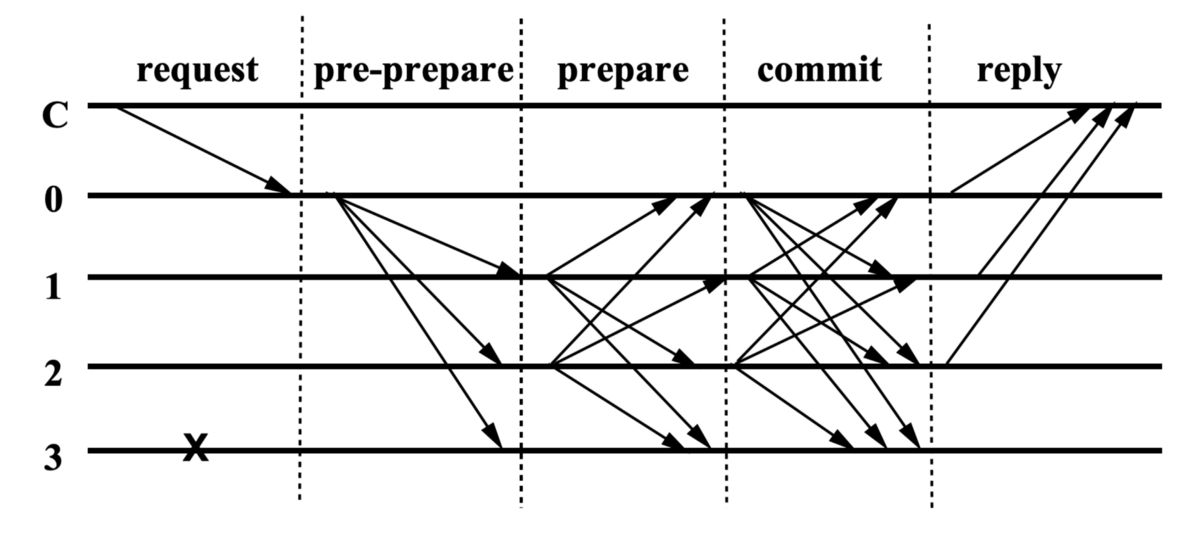
\includegraphics[width=4.5in, angle =0]{pbft}
	\caption{Flow of PBFT}
	\label{fig:pbft}
\end{figure}

\section{Blockchain Protocols}\label{sec:blockchain}

Blockchain protocols are a set of principles that regulate the security, recording, and sharing of data
within a blockchain network. A distributed ledger
maintains a continuously expanding list of records, or blocks, linked and secured using
cryptographic hashes. These blocks are connected in a chain
that is both tamper-evident and immutable, making it a great choice for applications that
needs trusted consensus among distributed participants.

Blockchain protocols are designed with the goal of achieving four key properties:
\begin{itemize}
  \item \textbf{Decentralization:} There isn't a single point of control or failure,
  data is replicated across multiple nodes.
  \item \textbf{Immutability:} Historical records of operations cannot be altered.
  \item \textbf{Transparency:} All transactions are visible to all participants.
  \item \textbf{Consensus:} All nodes maintain a consistent state despite potential Byzantine faults.
\end{itemize}

Blockchain systems are categorized into three main types based on access control and data
governance models~\cite{blockchain_consensus}:

\begin{itemize}
  \item \textbf{Public Blockchains (Permissionless):} In this type of blockchain, all participants can join without restrictions to
  validate transactions, and participate in consensus. These systems usually
  prioritize decentralization and censorship resistance while sacrificing performance and energy efficiency,
  especially when Proof of Work is used to achieve consensus like in Bitcoin, Ethereum, or Litecoin.

  \item \textbf{Private Blockchains (Permissioned):} These systems are characterized by a restricted controlled access for specific
  organizations or entities. Only authorized participants can join and participate in the network.
  These offer higher performance and privacy at the cost of decentralizing benefits.

  \item \textbf{Consortium Blockchains (Semi-decentralized):} In this model the network is
  controlled by a pre-selected group of participants, being it industry partners or allied organizations.
  These models usually achieve a balance between decentralization, performance, and regulatory compliance.
\end{itemize}

In this section, we will examine popular blockchain consensus protocols that address Byzantine
behavior under different system models and trust assumptions.

\subsection{Proof of Work (PoW)}\label{sub:pow}

The first blockchain protocol was achieved by
Proof of Work, introduced by Bitcoin~\cite{bitcoin} and adopted by Ethereum~\cite{ethereum} (pre-2022).
The next block producer is selected by this consensus mechanism through a computational competition
in which nodes (miners) compete to solve a mathematical puzzle with adjustable difficulty.

The PoW algorithm functions as follows: miners accumulate pending transactions into a block
candidate, and subsequently iteratively modify a nonce value while computing the block's hash
using a cryptographic function, like double SHA-256. The goal is to identify a hash that satisfies
the current difficulty target and automatically adjusts to preserve the average block time (e.g., 10 minutes for Bitcoin).

PoW offers a variety of security guarantees, including the longest chain rule, which
guarantees eventual consistency, requires that assailants control over 50\% of
the network's computational capacity for successful attacks, and the establishment of an
economic incentive structure through block rewards and transaction fees. However, this
comes at a cost of a large energy consumption and a restricted transaction throughput.

\begin{figure}[h]
	\centering
	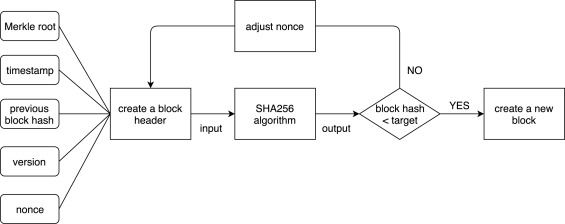
\includegraphics[width=4.5in, angle =0]{pow}
	\caption{Flow of PoW}
	\label{fig:pow}
\end{figure}

\subsection{Proof of Stake (PoS)}\label{sub:pos}

In Proof of Stake, nodes provide a stake that serves as the foundation
for consensus participation and block production rights, replacing the computational competition of PoW. 
Validators are chosen to generate new blocks in PoS based on the amount of their currency
they are willing to stake, rather than their computational power. This approach
considerably reduces energy consumption in comparison to Proof of Work protocols.
  
 A random selection function that is weighted by stake size is typically employed by
 the selection mechanism. Validators with larger stakes have proportionally higher odds of being
 selected to produce the next block. Modern PoS implementations like Ouroboros~\cite{ouroboros},
Ethereum 2.0's Gasper~\cite{gasper}, and Tendermint~\cite{tendermint} use selection algorithms
that provide cryptographic proofs of randomness and prevent tampering.

 Validators are required to deposit stakes as collateral in PoS systems, which can be
 partially or fully confiscated in the event of illegal activity, such as double-signing or
 violating protocol rules. This ensures that honest behavior is enforced through economic penalties.
 This achieves a higher transaction throughput and quicker finality than PoW systems, while also
 providing robust economic incentives for honest participation.

 Ethereum successfully transitioned from PoW to PoS in 2022, thereby illustrating the
 practical feasibility of this approach for large-scale blockchain networks. 

 Although Ethereum's transition to PoS was successful, it has exposed the
 protocols to vulnerabilities. In Section~\ref{sub:bouncing_attack}, one of these
 vulnerabilities will be further discussed.

\begin{figure}[h]
	\centering
	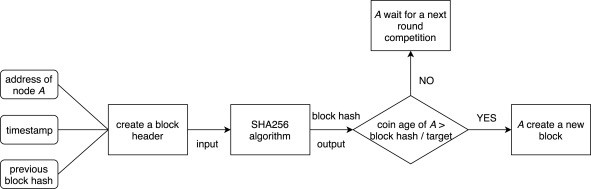
\includegraphics[width=4.5in, angle =0]{pos}
	\caption{Flow of PoS}
	\label{fig:pos}
\end{figure}


\subsection{Delegated Proof of Stake (DPoS)}\label{sub:dpos}

Delegated Proof of Stake introduces a representative democracy model,
in which token holders vote to elect a restricted number of delegates who are
responsible for network governance and block production.

In DPoS systems, token holders utilize their stake as a form of
voting authority to consistently elect delegates.
Compared to probabilistic consensus mechanisms such as PoW or traditional PoS, 
the top-voted delegates form a rotating committee that alternates in the production of blocks
in a round-robin fashion. This results in deterministic block latencies and a higher transaction throughput.

EOSIO~\cite{dpos_eosio}, Tron~\cite{dpos_tron}, and BitShares~\cite{bitshares} are all examples of DPoS implementations.
These protocols provide a variety of benefits, including a reduction in energy consumption, a higher
transaction throughput, and faster block confirmation periods, which typically range from one to three seconds.
This is achieved at the expense of centralization, as the system is susceptible to
censorship and collusion assaults due to the fact that only a small number of delegates have the ability to regulate block production.

Continuous voting ensures delegate accountability, as token holders have the ability to vote out delegates who
are performing inadequately or maliciously. This creates ongoing incentives for competent network operation
and honest behavior.

\begin{figure}[h]
	\centering
	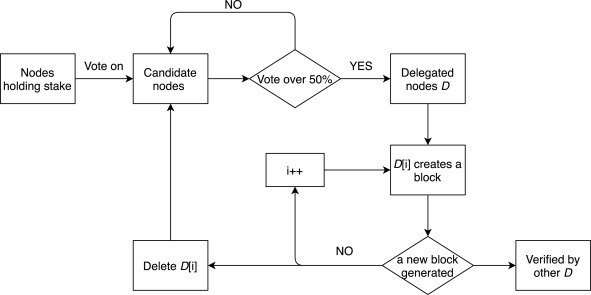
\includegraphics[width=4.5in, angle =0]{dpos}
	\caption{Flow of DPoS}
	\label{fig:dpos}
\end{figure}